% Kapitel 1
% Die Unterkapitel können auch in separaten Dateien stehen,
% die dann mit dem \include-Befehl eingebunden werden.
%-------------------------------------------------------------------------------

\chapter{Einleitung}
Die Datenbank WiReLib repräsentiert den Bestand der Bibliothek für das Institut für Wissenschaftliches Rechnen.
Auf diese Datenbank können Nutzer über ein Web-Interface zugreifen, um Dokumente zu suchen und sich nach der Anmeldung Dokumente auszuleihen.
Es gibt verschiedene Rollen, welche den Nutzern zugewiesen werden.
Die Verwaltung der Dokumente obliegt der Rolle des Bibliothekars.
Die Verwaltung der Benutzer obliegt der Rolle des Administrators.
Alle anderen Nutzer haben nur einfache Leserechte.
Die Anwendung wird nur im kleinem Rahmen eingesetzt und fungiert am Ende auf
Vertrauensbasis.

\section{Projektdetails}
Die Funktionalitäten gliedern sich in drei Teilbereiche.
Diese Bereiche bündeln die Anforderungen, die im Pflichtenheft spezialisiert
worden sind.

\begin{figure}[h]
\begin{center}
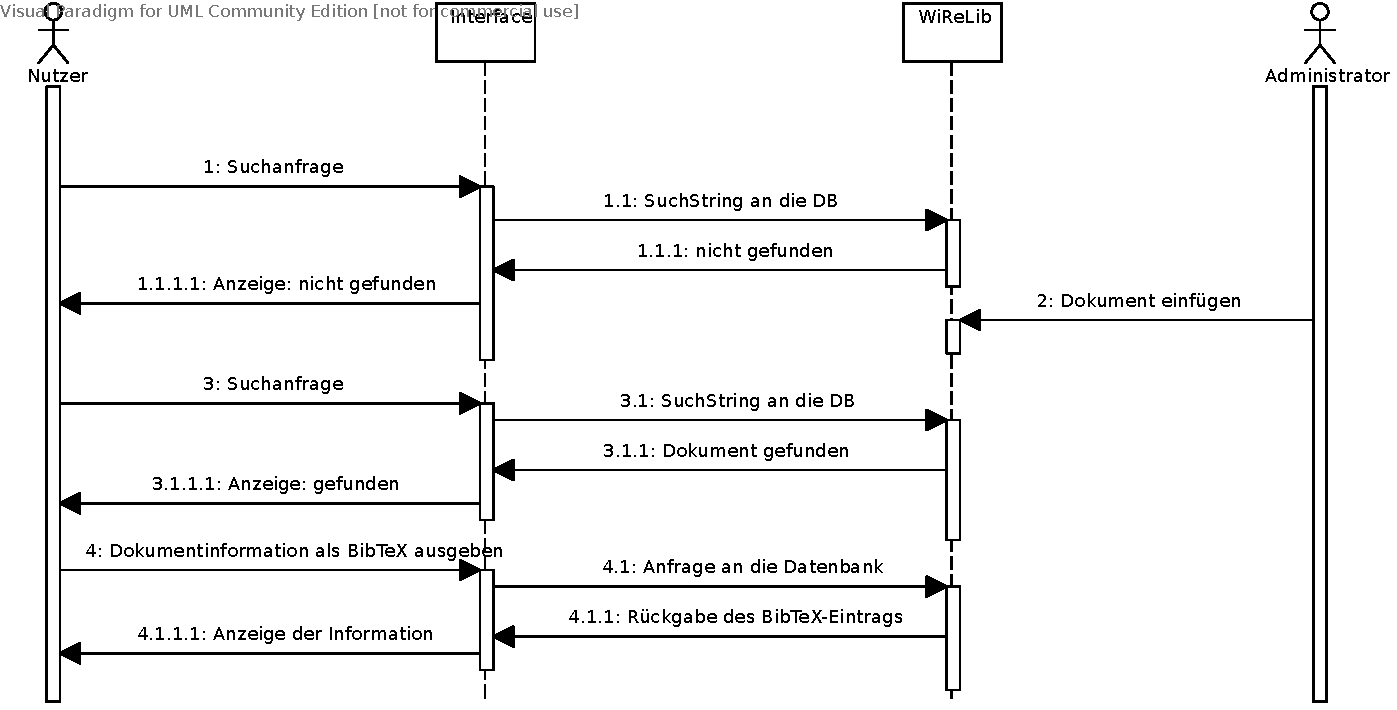
\includegraphics[width=0.9\linewidth]{bilder/Seq-Uebersicht.pdf}
\caption[Übersichtssequenzdiagramm]{Übersichtssequenzdiagramm}
\label{Seq-Übersicht}
\end{center}
\end{figure}

Im \ref{Seq-Übersicht} \nameref{Seq-Übersicht} werden grobe Abläufe im System 
veraunschaulicht um eine Übersicht über die Anwendung zu bekommen.
Da die Anmeldung zeitlich nicht festsetzbar ist und somit der Ausleih- und
Rückgabevorgang, werden sie nicht in diesem Diagramm dargestellt.

\subsection{Client}
Über das Web-Interface erhält der als Client fungierende Browser Zugriff 
auf die Datenbank.
Dort hat der Nutzer verschieden Funktionen zur Auswahl und kann sich zu den
Dokumenten, die in der Bibliothek vorhanden sind, Informationen ansehen.
Es wird wärend der Laufzeit keinerlei Speicher auf dem Client benötigt, da 
durch die Anwendung keine Daten auf dem Client gespeichert werden.

\subsection{Server}
Auf dem Server läuft die Anwendung, welche durch die Anwendung von Python und 
Django Code dynamisch HTML-Seiten generiert.
Sie stellt verschiedene Funktionen bereit, darunter Funktionen zum Auslesen 
und Verwalten der Datenbank. 
Auch stellt der Server die Datenbank bereit und baut eine sichere Verbindung 
zum Client auf.

\subsection{Datenbank}
In der Datenbank werden die Dokumente, sowie die Nutzerrechte verwaltet.
Auch werden Daten zu den einzelnen Nutzern gespeichert, um diese zu 
identifizieren und im Falle des Ablaufs der Verleihfrist mit einer E-Mail 
zu benachrichtigen.
Es wird auch der Status der Dokumente gespeichert, sowie an wen sie verliehen
wurden.
